\chapter{Diskussion der Umsetzung}
\label{chap:five}
\section{Design}
    \subsection{Technische Details der Implementierung}
    Der Entwurf des Proof-of-Concepts wurde mittels der Programmiersprache Python3 umgesetzt. 
    Python3 ist weitverbreitet, gut lesbar und gut dokumentiert. Genutzt wurde insbesondere die Python-Bibliothek 
    Pandas für den Datenimport und die Datenbearbeitung. Vor allem in Verbindung mit Pandas ist Python3 neben R und Matlab
    im wissenschaftlichen Kontext für Datascience-Projekte sehr beliebt. Pandas ist eine Open-Source-Bibliothek 
    für Datenanalyse und Datenmanipulation. Wichtige Konzepte dieser Bibliothek sind die des Dataframes und der Series. 
    Dataframe ist eine zweidimensionale tabellarische Datenstruktur mit beschrifteten Achsen (Spalten und Reihen).
    Währenddessen eine Pandas Series ein eindimensionales Array darstellt. Auf dem Dataframe, das als sogenannter Container für
    die geladenen Daten aus csv oder xlsx-Dateien dient, können dann verschiedene Operationen der Datenanalyse und -manipulation erfolgen.

    
    Für die Erstellung der Datenvisualisierungen wurde die Bibliothek Plotly Express genutzt. 
    Das Dashboard wurde mit dem Framework Dash entwickelt, mit welcher die Diagramme leicht eingebunden. 
    Sowohl Plotly Express als auch Dash werden von derselben Firma entwickelt. Dash baut
    auf Flask, Plotly.js und React.js auf. Das Framework ermöglicht, die Erstellung interaktiver Webapplikationen 
    in reinem Python ohne Kenntnisse von Javascript und mit wenig Wissen von HTML und CSS. \autoref{tab:Software-Requirements} zeigt einen 
    kurzen Überblick über die Versionsnummern der genutzten Programmiersprache und der Frameworks sowie deren Open-Source
    Lizenzen.
    
    \begingroup
        \setlength{\tabcolsep}{4pt} % Default value: 6pt
        \renewcommand{\arraystretch}{1.5}
        %\resizebox{\textwidth}{!}{
        \begin{table}[h]
            \centering
            \begin{adjustbox}{max width=\textwidth}
            \Huge
            \begin{tabular}{lccl}
              %\begin{tabular}{p{3cm}p{5cm}p{1cm}p{1.5cm}p{2cm}p{4cm}}
               \toprule
               \textbf{Name}             &{Version}    &\textbf{Lizenz}                        & \textbf{Webseite}\\
               \midrule     
                    Python               &3.7.9         &Open Source (PSF)                     & \url{https://docs.python.org/3.5/}\\
                    Pandas               &1.1.2         &3-Clause-BSD-License                  & \url{https://pandas.pydata.org/pandas-docs/version/1.1.2/}\\
                    Plotly Express       &0.4.0         &MIT-License                           & \url{https://plotly.com/python/}\\
                    Dash                 &1.16.3        &MIT-License                           & \url{https://dash.plotly.com/}\\


                \bottomrule
            \end{tabular}
            \end{adjustbox}
            \caption
            \label{tab:Software-Requirements}
            }
             \end{table}
        \endgroup
    
     
    \subsection{Systemarchitektur}
    
    Das System teilt sich in XX Teilsysteme auf. \autoref{tab:Teilsysteme} zeigt die XX Teilsysteme mit einer Kurzbeschreibung.
    Objekt-orientiert programmiert wurden ebenso nur Teile des Systems. Diese Teile sind der Bereich des Datenimports, der Datenberechnung. Wohingegen die Bereiche der            
    Darstellung mit dem Dashframework nicht mehr objektorientiert im Rahmen dieser Arbeit umgesetzt werden konnte.
    
       \begingroup
            \setlength{\tabcolsep}{4pt} % Default value: 6pt
            \renewcommand{\arraystretch}{1.5}
            %\resizebox{\textwidth}{!}{
            \begin{table}[h]
                \centering
                \begin{adjustbox}{max width=\textwidth}
                \Huge
                \begin{tabular}{lccl}
                  %\begin{tabular}{p{3cm}p{5cm}p{1cm}p{1.5cm}p{2cm}p{4cm}}
                   \toprule
                   \textbf{Teilsystem}             &{Hauptaufgabe} \\
                   \midrule     
                        Import               &Import und Transformation der Daten aus heterogenen Datenquellen.\\
                        Datenbearbeitung     &Aufbereitung der Daten für die graphische Darstellung im Dashboard.\\
                        Darstellung          &Bereitstellung der Daten und Anzeige der Daten im Dashboard.\\
                        Standardbericht      &Export ausgewählter Datenvisualisierungen und Darstellung in Berichtsform.\\

                    \bottomrule
                \end{tabular}
                \end{adjustbox}
                \caption
                \label{tab:Teilsysteme}
                }
                 \end{table}
            \endgroup
    



    

% Urls zu den als Fußnoten dazufügen.

Herausfiltern der Datensätze zum Beispiel aus den Neuerwerbungslisten, hinter denen keine physische Entsprechung zum einen steht (mehrteilige Ressouurce auf Gesaamtitel?ebene, Datensätze Schriftenreihen)

    
    
    grobes Bild der Systemarchitekturmit Klassen -> UML-Diagramm mit Bereichen
    
    
    Plotly Express\\
    Pandas\\
    Dash\\
    -> effizient und effektiv zu sein




    \begin{lstlisting}[language=Python, caption=Python example]
        import pandas as pd
        import plotly.express as px

        
    \end{lstlisting}

    \subsection{Teilsysteme}
    
    Import-System\\
    Das Import-System ist verantwortlich für den Import der Daten im Rohformat aus einem definierten Importverzeichnis in ein definiertes Zielverzeichnis. Das Ziel
    ist einerseits die Daten ohne Informationsverlust zu importieren und und andererseits diese mit notwendigen Daten anzureichern. Die Daten werden in ein Pandas Dataframe
    geladen. Dort finden die notwendigen Transformationen (Clean, Add) statt. Dieses veränderte Dataframe wird am Schluss des Prozesses in eine csv-Datei umgewandelt.
    
    Die Klassen im Import Module sind auf den Daten aus fremden Quellen zugeschnitten.
    (Budget Umsatz, Neuerwerbungslisten (Anwendungsfall 4 - 6))
    Ziel: Die Daten ohne Verluste zu importieren. Dabei spielt für die spätere Anwendung im System, der mtl. Stand
    ausgedrückt im Datum eine wichtige Rolle.
    Es wurden als Datengrundlage nur die Daten berücksichtigt, die für die Anwendungsfälle benötigt werden.
    Außen vor blieb zum Beispiel die Integration der Counter-Daten.
    Die von der Bibliothek erhobenen Daten.
    
    Die allgemeine Funktionsweise des Teilsystems zeigt die \autoref{fig:flow import}.

    \begin{figure}[H]
        \centering
            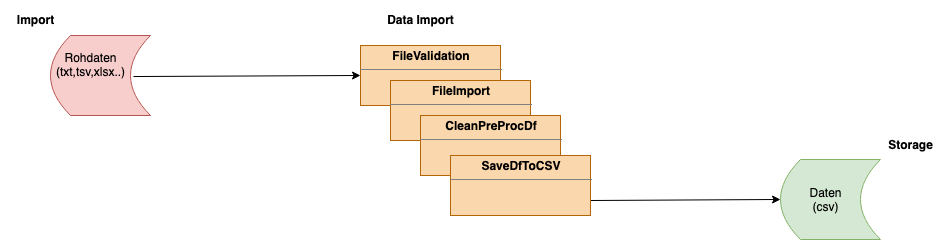
\includegraphics[width=12cm, height=2.5cm]{flow_imp}
            \caption{Datenfluss - Teilsystem Import}
            \label{fig:flow import}
    \end{figure}
    
    Die \autoref{fig:classes import} zeigt die einzelnen Klassen mit ihren Methoden des Teilsystems.

    \begin{figure}[H]
        \centering
            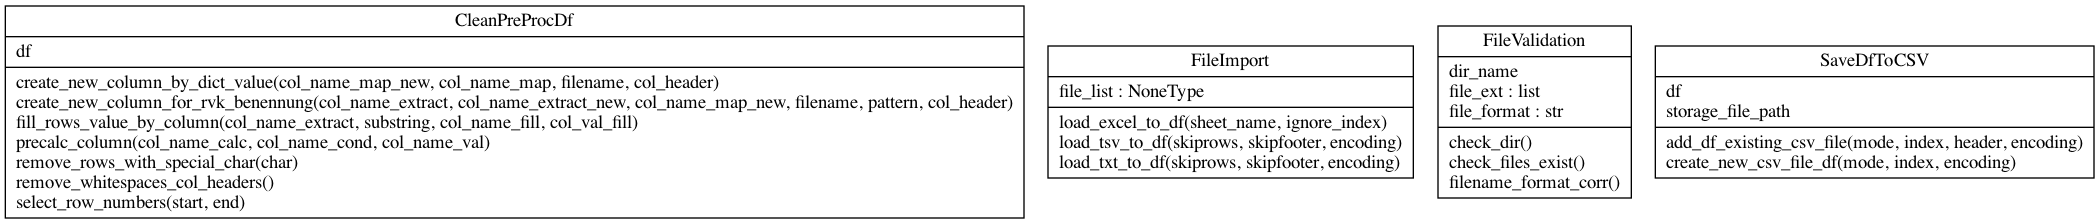
\includegraphics[width=14cm, height=2.5cm]{classes_imp}
            \caption{Klassendiagramm - Teilsystem Import}
            \label{fig:classes import}
    \end{figure}
    
    (1) Für Schritt 1 sind die Klassen FileValidation und FileImport verantwortlich.
    Die Dateien werden aus einem vorher definierten lokalen Verzeichnis in ein Pandas Dataframe exportiert. Dabei wird mit Methoden
    der Klasse FileValidation sichergestellt, dass sowohl das Verzeichnis als auch die Dateien existieren. Des Weiteren wird sichergestellt,
    dass die Dateinamen einem definierten semantischen Format entsprechen (z.B. YYYY\_MM\_DD.txt). 
    Da die Daten unterschiedlich aufgebaut und in unterschiedlichen Dateiformaten vorliegen werden beim Import in den Dataframe jeweils verschiedene Methoden angewandt. Je
    % nachdem welches Format vorliegt, wird aus den drei Methoden load\_txt\_to\_df, load\_tsv\_to\_df oder load\_excel\_to\_df der Klasse FileImport ausgewählt .
    Beim Ladeprozess in den Dataframe wird mit den Methoden load\_txt\_to\_df oder load\_tsv\_to\_df der Klasse FileImport beim Import der Datei in den Dataframe der Dateiname
    extrahiert und in eine neue Spalte des Dataframe als String im Datumsformat YYYY-MM-DD gespeichert. Die neu entstandene Spalte ist für die spätere Auswertung und
    Darstellung der Daten im Dashboard wichtig, da anhand der Spalte die Daten nach dem Datum ausgewertet werden können.\footnote{Dieses Verfahren wurde bei Daten eingeführt
    bei denen es einer zusätzlichen Datumsspalte bedurfte Umsatz,
    Budget und Neuerwerbungen die als txt oder tsv-Daten im Originalformat vorliegen.} Verantwortlich für die Umwandlung des Dateinamens in einen String ist die in utils.py
    ausgelagerte Funktion date\_from\_filename, die den Dateinamen als Parameter entgegennimmt. 
    
    (2) Für Schritt 2 ist die Klasse CleanPreprocDF verantwortlich. 
    Anschließend können noch verschiedene Methoden der Klasse CleanPreProcDF auf das Dataframe zur Anwendung kommen. Hervorzuheben wäre hier die Methode 
    create\_new\_column\_for\_rvk\_benennung, die aus der Spalte der Signatur der Neuerwerbungen die Hauptklassen der RVK extrahiert. Zusätzlich liegt dieser Methode eine csv-Datei
    der RVK (ergänzt um spezifische Hauptklassen der Institutsbibliothek) zu Grunde, die zuerst in ein Dictionary eingelesen wird und dann werden die Keys (Hauptklasse) mit den
    extrahierten Hauptklassen gemapt und eine neue Spalte mit den values (Benennung) der Hauptklassen im Dataframe angelegt.    
    
    
    (3)  Für Schritt 3 ist die Klasse SaveDfToCSV verantwortlich.
    Nachdem Transformationsprozess wird dsa veränderte Dataframe als csv-Datei in einem vorher definierten Zielordner gespeichert. Verantwortlich ist dabei die Klasse    
    SaveDFToCSV mit den zwei Methoden add\_df\_existing\_csv\_file create\_new\_csv\_file\_df. Die jenach dem mit dem Dataframe eine neue csv-Datei kreiren oder an eine bereits       
    vorhandene csv-Datei den Dataframe anhängen.
    
    Den Transformationsprozess vom Originalzustand als txt-Datei in den gewünschten Zustand als csv-Datei zeigt die Abbildung XX exemplarisch für den Umsatz bei den
    Lieferanten. (wide or long form-tabelle)
    
    Bild einfügen
    
    
    Das Import-System ist verantwortlich für den Import der Daten im Rohformat aus einem definierten Importverzeichnis in ein definiertes Zielverzeichnis. Das Ziel
    ist einerseits die Daten ohne Informationsverlust zu importieren und und andererseits diese mit notwendigen Daten anzureichern. Die Daten werden in ein Pandas Dataframe
    geladen. Dort finden die notwendigen Transformationen (Clean, Add) statt. Dieses veränderte Dataframe wird am Schluss des Prozesses in eine csv-Datei umgewandelt.
    Einbindung der RVK-Systematik - gewisse Anpassung durch die Bibliothek -> Hinzunahme von eigenen Systematikstellen,
    
    die zum Teil andere Systematikstellen ersetzten (NT eigentlich Rechtswissenschaften, in der Institutsbibliothek Noten, MT eigentlich
    Gesundheitswissenschaften, in der Institutsbibliothek Methoden)
 
      
    Kurzbeschreibung / Ziel:\\
    Wo zu finden:\\
    Datengrundlage:\\
    Klassenbeschreibung:\\
    Prozess:\\
    
    Grafik
    
    Klassenbeschreibung: mit Methoden und evtl. Funktionen
    Das System splittet sich in XX Teilsysteme auf: Import-System, Datentransformtion und Datenhaltung, Diagramme, Dash, PDF-System. Dazu gibt es noch Skripte,
    die der Datenextraktion dienen. Diese sind zu finden in dem Ordner XX. Notwendige andere Dateien, die die Auswahll der angezeigten daten steuern sind zu finden im          
    Verzeichnis: XX
    
    Abbildung: UML-Diagramm mit Bereichen
    
    
    Import-System\\
    Das Import-System ist verantwortlich für den Import der Daten im Rohformat aus einem definierten Importverzeichnis in ein definiertes Zielverzeichnis. Das Ziel
    ist einerseits die Daten ohne Informationsverlust zu importieren und und andererseits diese mit notwendigen Daten anzureichern. Die Daten werden in ein Pandas Dataframe
    geladen. Dort finden die notwendigen Transformationen (Clean, Add) statt. Dieses veränderte Dataframe wird am Schluss des Prozesses in eine csv-Datei umgewandelt.
    
    
    Während des Imports werden 
    die monatlichen Daten aus dem Rohformat (tsv, txt-Dateien), bereinigt, vorverarbeitet und in ein einheitliches csv-Format umgewandelt. Dabei werden neue Spalten für das
    Datum aus dem Dateinamen, der in einer vorher definierten semantischen Form vorliegen muss, für Budget- und Umsatzdaten und für Neuerwrbungsdaten erzeugt. Zudem wird aus
    den Signaturen der Neuerwerbungen in den Daten zusätzliche Spalten erzeugt. Diese neugewonnenen Spalten dienen der späteren Analyse und Darstellung der Daten im Dashboard.
    Kurzbeschreibung / Ziel: Import der Daten aus einem lokalen Folder in einen anderen . 
    Die Daten ohne Verluste zu importieren. Dabei spielt für die spätere Anwendung im System, der mtl. Stand ausgedrückt im Datum eine wichtige Rolle.\\
    Wo zu finden: Modul XX im Folder \\
    Datengrundlage: Es wurden als Datengrundlage nur die Daten berücksichtigt, die für die Anwendungsfälle benötigt werden.
    Außen vor blieb zum Beispiel die Integration der Counter-Daten.
    Budget, Umsatz, Ausleihdaten, Neuerwerbungslisten in txt, tsv-Formaten.
 
 
 
 
 
 
 
 
 
 
    Klassenbeschreibung:
    Prozess: Die Klassen im Import Module sind auf den Datenbestand aus fremden Quellen zugeschnitten.
    (Budget Umsatz, Neuerwerbungslisten (Anwendungsfall 4 - 6))
    Add: Datum bei Budget, Umsatz-Daten, Ausleihdaten, evtl. RVK-Systematikstelle, das wichtig ist für spätere Auswertung und grafische Darstellung
    im Dashboard
  
  
    Import der Daten aus einem lokalen Folder in einen anderen. 
    Währenddessen Bearbeitung der Daten und Basic Cleaning
    Umsetzung:
    Add: Datum bei Budget, Umsatz-Daten, Ausleihdaten, evtl. RVK-Systematikstelle 
    Die Klassen im Import Module sind auf den Datenbestand aus fremden Quellen zugeschnitten.
    (Budget Umsatz, Neuerwerbungslisten (Anwendungsfall 4 - 6))
    Ziel: Die Daten ohne Verluste zu importieren. Dabei spielt für die spätere Anwendung im System, der mtl. Stand
    ausgedrückt im Datum eine wichtige Rolle.
    Es wurden als Datengrundlage nur die Daten berücksichtigt, die für die Anwendungsfälle benötigt werden.
    Außen vor blieb zum Beispiel die Integration der Counter-Daten.
    Die von der Bibliothek erhobenen Daten. Die Übersicht zeigen folgende Methoden der einzelnen Klassen.
    git
    

\section{Implementierung}

  

    \subsection{Umgesetzte Anforderungen}
    Folgende Must-Anforderungen wurden erfüllt.
    R1, R2, R3, R4, R5, R7
    F1, F4, F5, F12
    NF5, NF6, 
    \subsection{Funktionsweise}
    Das Layout des Dashboards besteht aus drei Tabs. Diese wurden nach den XXX Berreichen der Bibliothek aufgeteilt. Diese Aufteilung eerschien als sinnvoll,
    da hier nichts überfrachtet wird.

    Beim Import werden zum beispiel txt-Dateien für das Budget und den Umsatz nach Lieferanten importiert von einem lokalen Verzeichnis
    in ein Zielverzeichnis importiert. Nach Abschluß des Prozesses liegen die Daten im csv-Format vor und sehen so aus wie in Abbildung
    old -> new
    figure
    
     



\section{Bewertung}
